Revealed high-frequency terms like number, url, date, mail, list, get, time, system, use, and HTML-related terms
(font, nbsp, td, tr).
The prevalence of number and url might indicate preprocessing/anonymization or simply be features of the emails.
HTML terms suggest formatted emails are common.

\begin{figure}[H]
    \centering
    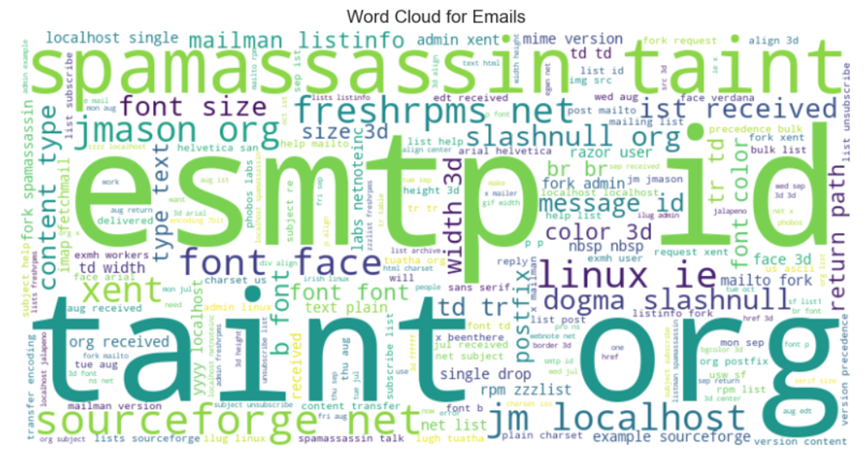
\includegraphics[width=\linewidth]{images/word_cloud}
    \caption{All emails in the form of Word Cloud}
    \label{fig:word_cloud}
\end{figure}

\smallskip
Prominent Keywords:

\begin{itemize}
    \item taint, spamassassin, esmtp, org, id, localhost, net, sourceforge: These are the largest and boldest words,indicating they are the most frequent and important terms within the analyzed email data.
    \item The rest of the word cloud: These words are smaller but still noticeable,suggesting they also play a significant role in the email context.
\end{itemize}

Possible Suggested Topics:

\begin{itemize}
    \item Spam Filtering: The presence of ``spamassassin'' and ``taint'' (often associated with marking suspicious emails) suggests a significant topic might be the identification and handling of spam.
    \item Mailing List Management: Words like ``list'',``listinfo'', ``mailman'', and ``mailing'' hint at discussions related to managing and interacting with email lists.
    \item Technical Email Information: Terms such as ``smtp'' (Simple Mail Transfer Protocol), ``mime'' (Multipurpose Internet Mail Extensions), ``version'',``id'', ``localhost'', and ``net'' indicate potential discussions about the technical aspects of email.
    \item Formatting and Display: Words like ``font'',``size'', ``face'', ``text'', and ``color'' might relate to how emails are displayed and formatted.
    \item Source and Path: ``sourceforge'' (an open-source software repository), ``received'', and ``path'' could be related to tracking the origin and route of emails.
    \item Related Systems and Software: ``linux'', ``xent'', and ``rpm'' might be the names of operating systems or software mentioned within the email context.
\end{itemize}